\subsubsection{Overview}
\label{Wang-Buzsaki Neuron}
\index{Wang-Buzsaki}\index{utilities, Wang-Buzsaki Neuron}
\begin{figure}[h]
\begin{center}
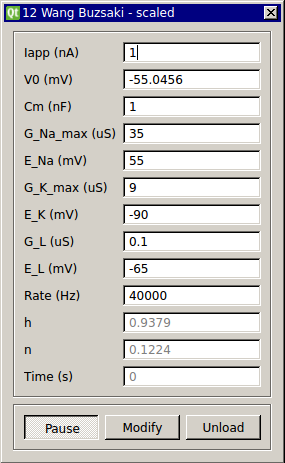
\includegraphics[width=2in]{wbneuron.png} 
\caption[WB Neuron]{GUI for a real-time Wang-Buzsaki neuron within RTXI.} 
\end{center}
\label{wbneuron}
\end{figure}

The Wang-Buzsaki model uses the Hodgkin-Huxley formalism to describe a single-compartment neuron with sodium and potassium conductances. For the transient sodium current, the activation variable m is assumed fast and substituted by its steady-state function.

Wang XJ, Buzsáki G (1996) Gamma oscillation by synaptic inhibition in a hippocampal interneuronal network model. J. Neurosci. 16: 6402–6413.

\subsubsection{Input Channels}
\begin{description}
\item[input(0)- Istim] input current (A)
\end{description}

\subsubsection{Output Channels}
\begin{description}
\item[output(0) - Vm] membrane voltage (V)
\end{description}

\subsubsection{Parameters}
\begin{description}
\item[Iapp] applied current (nA)
\item[V0] voltage (mV)
\item[Cm] membrane capacitance (nF/cm\^2)
\item[G\_Na\_max] max. Na+ conductance density  (uS/cm\^2)
\item[E\_Na] Na+ reversal potential (mV)
\item[G\_K\_max] max. K+ conductance density (uS/cm\^2)
\item[E\_K] K+ reversal potential (mV)
\item[G\_L] leak channel conductance density (uS/cm\^2)
\item[E\_L] leak channel reversal potential (mV)
\item[rate] rate of integration (Hz)
\end{description}

\subsubsection{States}
\begin{description}
\item[h] sodium inactivation
\item[n] potassium inactivation
\item[Time] time (s)
\end{description}